\documentclass[11pt,titlepage]{report}
\usepackage{Preamble}
\addbibresource{ref.bib}

\begin{document}

\begin{titlepage}
	\newgeometry{margin=3cm}
	\centering
    \includegraphics[width=0.75\linewidth]{hes/hei}\\[1cm] 	% University Logo
    \textsc{\LARGE Haute école d'ingénieur du Valais}\\ \vspace{\fill}
    \textbf{\textsc{\fontsize{35}{35}\selectfont SuperLab - XF}}\\ \vspace{\fill}
	\textsc{\LARGE Real Time Programming}\\[0.4cm]
	\rule{\linewidth}{0.2 mm}\\[0.5cm]
	Samy Francelet \\
	\today
\end{titlepage}
\restoregeometry

\tableofcontents

\chapter{Introduction}
\begin{summary}
\section{Contexte}
Ce laboratoire a servi d'introduction à la programmation temps réel sur
système embarqué (ici STM32).
Le but était d'implémenter un Execution Framework (XF), en architecture IDF (sans
couche RTOS) pour simplifier le développement.
Notre XF se doit d'être portable, avec une implémentation sur PC avec
la librairie Qt, et une autre sur système embarqué STM32. Des tests communs aux deux
systèmes sont fournis, ainsi qu'une structure de base du projet.
\end{summary}

\section{XF}
Le XF (execution framework) est un framework servant à piloter plusieurs machines
d'états finies en pseudo-parallèle. Pour cela, il utilise des événements qui sont générés
par les machines d'états, qui passent par un Dispatcher avant d'être redistribué.
\begin{figure}[H]
    \centering
    \includegraphics[width=0.75\textwidth]{Images/xf/IDF.PNG}
    \caption[Schéma de principe de notre XF en IDF]{Schéma de principe de notre XF en IDF (provenant du \emph{Cours XF}\footnotemark)}
\end{figure}
\footnotetext{\cite{coursXF}}
Dans notre cas, le XF fonctionnera directement sur le hardware, et tournera grâce
aux interruptions systèmes (architecture IDF). Ce cas est opposé d'un XF tournant
par-dessus un Real Time OS (architecture OXF). L'implémentation est plus simple, mais 
l'efficacité à grande échelle est réduit.

\begin{figure}[H]
    \centering
    \includegraphics[width=\textwidth]{Images/xf/comp-simple-xf.png}
    \caption[Diagramme de composant de classe du XF]{Diagramme de composant de classe du XF 
        (provenant de la documentation \emph{Simplified XF}\footnotemark)}
\end{figure}
\footnotetext{\cite{documentation}}
Notre implémentation du XF se veut portable. Il a donc était séparé en deux parties :
\begin{itemize}
    \item XF::Core -> Contient le cœur du XF (machines d'état, événements), 
            cette partie restera inchangée sur tous les systèmes.
    \item XF::Port -> Contient les différents ports du XF, certains de ses ports
            seront spécifiques à chaque système (ex: XFMutex qui bloque les interruptions 
            sur système embarqué, et qui est un Mutex classique sur PC)
\end{itemize}
Le cœur et les ports forment ensemble un XF complet.
La majeur partie du XF::Core est déjà implémentée. Les événements restent à préciser.

\chapter{Conception}
\section{Board Layer}
Après une configuration de la board réalisé avec \emph{STM32CubeMX} (détail
de la configuration dans le \emph{Guide ButtonsController}\footnotemark[1])
Dans la \emph{Board Layer}, la machine d'état du \emph{ButtonsController}
est implémentée.
\begin{figure}[H]
    \centering
    \includegraphics[width=0.45\textwidth]{Images/buttons/btnCtrl.PNG}
    \caption[Full UML]{State diagram du BoutonsController (provenant du \emph{Guide ButtonsController}\footnotemark[1])}
\end{figure}
\footnotetext[1]{\cite{lab_guide}}
Le fonctionnement de cette couche est simple : une interruption Hardware enclenche
le \emph{STATE\_DEBOUNCE}. Après 100 millisec, on retourne dans l'état d'attente,
et on contrôle l'état de tous les boutons. Ce temps d'attente permet de réaliser un
anti-rebond software.\newpage

\section{Middleware Layer}
Le \emph{Middleware} implémente la détection d'appui court ou long sur un bouton.
Elle reçoit les informations de la \emph{Board Layer} pour son fonctionnement, et
transmet les informations d'appui court ou long à la couche \emph{Application}
\subsection{Liaison avec la Board Layer}
La liaison avec la couche en dessous ce fait ainsi :
\begin{figure}[H]
    \centering
    \includegraphics[width=0.75\textwidth]{Images/buttons/mdw_layer.PNG}
    \caption[Full UML]{Diagramme de classe du mdw (provenant du \emph{Guide ButtonsController}\footnotemark[1])}
\end{figure}
\footnotetext[1]{\cite{lab_guide}}
Le \emph{ButtonEventsHandler} implémente l'interface \emph{ButtonsControllerCallbackProvider}
pour fournir la méthode \textbf{onButtonChanged} en méthode de callback.
La méthode de callback sera appelée par le \emph{ButtonsControllerCallbackCaller}.
Cela permet donc au \emph{ButtonsController} d'informer le \emph{ButtonEventsHandler}
d'un changement sur un bouton, sans aucune liaison direct entre les deux classes.
\newpage

\subsection{ButtonEventsHandler}
Le gestionnaire d'évenement boutons \emph{ButtonEventsHandler} fonctionne ainsi :
\begin{figure}[H]
    \centering
    \includegraphics[width=0.3\textwidth]{Images/buttons/btnEvHandler.PNG}
    \caption[Full UML]{Diagramme de classe du \emph{ButtonEventsHandler}
    (provenant du \emph{Guide ButtonsController}\footnotemark[1])}
\end{figure}
Lorsqu'il reçoit une information sur un bouton, il transmet un évenement
au \emph{ButtonStateSM} correspondant. Chaque \emph{ButtonStateSM} possède
une machine d'état interne :
\begin{figure}[H]
    \centering
    \includegraphics[width=0.75\textwidth]{Images/buttons/btnSM.PNG}
    \caption[Full UML]{Diagramme d'état d'un \emph{ButtonStateSM}
    (provenant du \emph{Guide ButtonsController}\footnotemark[1])}
\end{figure}
\footnotetext[1]{\cite{lab_guide}}
La machine d'état reçoit l'évenement \textbf{evButtonPressed}.
Une fois à l'état pressé, si le bouton est relaché avant 1 sec, elle notifie
le \emph{ButtonEventsHandler} d'un appui court, sinon d'un appui long.\newpage

\section{Application Layer}
\subsection{Liaison avec le Middleware}
\begin{figure}[H]
    \centering
    \includegraphics[width=0.75\textwidth]{Images/buttons/app_layer.PNG}
    \caption[Full UML]{Diagramme de classe de l'App (provenant du \emph{Guide ButtonsController}\footnotemark[1])}
\end{figure}
\footnotetext[1]{\cite{lab_guide}}
Pour permettre d'ajouter plusieurs module a la couche \emph{Application},
un patterne \emph{Subject - Observer} a été utilisé.
Le \emph{ButtonEventsHandler} possède une liste d'\emph{Observer}, a qui il
va notifier les appuis longs ou court. Les \emph{Observers} vont pouvoir
\textbf{subscribe} au \emph{Subjet} pour informer qu'ils souhaitent être notifié
des évenement boutons.
\subsection{Découplage complet du ButtonEventsLogger}
Pour découpler "totalement" le \emph{ButtonEventsLogger}, il a été demandé
d'en faire une machine d'état.
\begin{figure}[H]
    \centering
    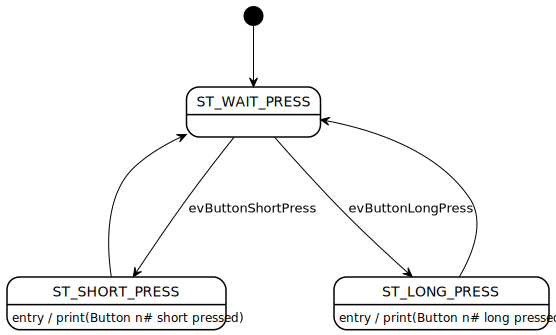
\includegraphics[width=0.6\textwidth]{Images/buttons/ButtonEventsLogger.png}
    \caption[Full UML]{Diagramme d'état du \emph{ButtonEventsLogger}}
\end{figure}\newpage

\subsection{ButtonEventsLedFlasher}
Le \emph{ButtonEventsLedFlasher} transmet les évenement \textbf{evButtonShortPress} et 
\textbf{evButtonLongPress} à des machines d'états \emph{LedStateSM} :
\begin{figure}[H]
    \centering
    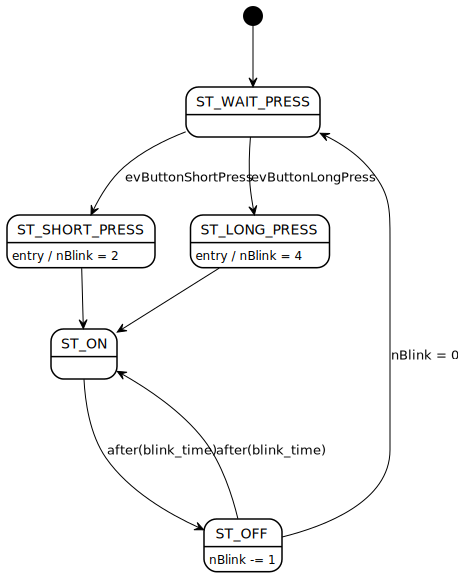
\includegraphics[width=0.5\textwidth]{Images/buttons/LedsStateSM.png}
    \caption[Full UML]{Diagramme d'état d'une \emph{LedStateSM}}
\end{figure}
Ces machines d'états appellent ensuite des méthode du \emph{LedsController} fournit
dans les modules de base.

\chapter{Résultats et tests}
\section{Description des test}
5 bancs de test ont été définis pour tester différents comportement du XF.
Ces 5 bancs de tests sont disponibles sous Qt, et sous STM32 avec STM32CubeIDE.
\subsection{Test-bench 1}
Le premier test instancie 2 machines d'états générant des timeouts, puis
transmettant une phrase à chaque timeout : un premier transmet "Say Hello" chaque
seconde, le second: "Echo" chaque 500ms.

\subsection{Test-bench 2}
Le second test instancie deux machines d'état identique, à l'exception qu'une
est un objet dynamique (et donc destructible).
Les deux objets vont passé un décompte de 5, avant d'être terminé. L'objet dynamique
devra être détruit et son destructeur devrait afficher "Called destructor".

\subsection{Test-bench 3}
Ce test check la gestion basique des événement dans les machines d'état.
Une machine d'état s'envoie périodiquement à elle même un "evRestart" pour
passer d'un état à l'autre.

\subsection{Test-bench 4}
Génère plusieurs timeout, puis crée un restart, qui devra unschedule des timeouts.
Si ce test n'est pas réussi, la liste des timeouts devrait se remplir, et on
aurait des comportements étranges.

\subsection{Test-bench 5}
Transmets plusieurs timeout en même temps au Timeout Manager pour stress-test l'ajout
intelligent de timeouts.

\section{Discussion des résultats}
Tous les tests ont été validés sur les deux systèmes. Le timing du système embarqué
est compliqué à mesurer. Nous utilisons le port série pour communiquer les
textes au PC, qui va stocker dans un buffer les données et les sortir quand il
pourra, donnant des timings étant parfois 20ms en avance, des fois 20ms en retard.
Les timings fournis en Annexe B seront donc uniquement les timings mesurer avec Qt.

%\chapter{Discussions}
%\input{4-Discussion}

\chapter{Conclusion}
\section{Bilan}
Le programme fonctionne parfaitement, toutes les méthodes de debounce, découplage,

\begin{summary}
\section{Conclusion personnelle}
Ce projet a permis de se rendre compte de l'importance du découplage
et des patternes. L'ajout du \emph{ButtonEventsLedFlasher} a été
extrêmement simple une fois l'intégralité du programme opérationel.
\end{summary}

\section{Signature}
Samy Francelet

\appendix
\chapter{Diagrammes de classe}
\begin{figure}[H]
	\centering
	\includegraphics[angle=90, height=0.7\textheight]{Images/xf/comp-simple-xf.png}
\end{figure}

\begin{figure}[H]
	\centering
	\includegraphics[angle=90, height=\textheight]{Images/xf/cmd-simple-xf.png}
\end{figure}

\chapter{Tests}
\section{Test 1}
\begin{figure}[H]
	\centering
	\includegraphics[]{Images/tests/test1.PNG}
\end{figure}

\section{Test 2}
\begin{figure}[H]
	\centering
	\includegraphics[]{Images/tests/test2.PNG}
\end{figure}

\section{Test 3}
\begin{figure}[H]
	\centering
	\includegraphics[]{Images/tests/test3.PNG}
\end{figure}

\section{Test 4}
\begin{figure}[H]
	\centering
	\includegraphics[]{Images/tests/test4.PNG}
\end{figure}

\section{Test 5}
\begin{figure}[H]
	\centering
	\includegraphics[]{Images/tests/test5.PNG}
\end{figure}


\printbibliography[heading=bibintoc]

\end{document}
